\documentclass[11pt, oneside]{scrreprt}   	% use "amsart" instead of "article" for AMSLaTeX format
\usepackage{geometry}                		% See geometry.pdf to learn the layout options. There are lots.
\geometry{letterpaper}                   		% ... or a4paper or a5paper or ... 
%\geometry{landscape}                		% Activate for rotated page geometry
%\usepackage[parfill]{parskip}    		% Activate to begin paragraphs with an empty line rather than an indent
\usepackage{graphicx}				% Use pdf, png, jpg, or eps§ with pdflatex; use eps in DVI mode
								% TeX will automatically convert eps --> pdf in pdflatex		
\usepackage{amssymb}
\usepackage{amsmath,amsfonts,amsthm} % Math packages
\usepackage{bm}
\usepackage{subcaption}
\usepackage{graphicx}
\graphicspath{ {images/} }


%%%%%%%%
%    Cover     %
%%%%%%%%
\title{\textit{}\\\textit{}\\State Space Models}
\author{Hans-Peter H{\"o}llwirth}
\publishers{Master Project Report \\ 
Barcelona Graduate School of Economics \\ Master Degree in Data Science \\ 2017}
\date{}

\begin{document}
\maketitle
%\afterpage{\blankpage}

%%%%%%%%%%%%%
%    Table of Contents   %
%%%%%%%%%%%%%
\newpage
\tableofcontents
\newpage

%%%%%%%%%%
%    Introduction   %
%%%%%%%%%%
\chapter{Introduction}
\label{chp:introduction}



%%%%%%%%
%    Models   %
%%%%%%%%
\chapter{State Space Models}
\label{chp:models}
State space models consist of two series of data:
\begin{enumerate}
	\item A series of latent \textbf{states} $\{x_t\}$ forming a Markov chain. Thus, $x_t$ is independent of all past states but $x_{t-1}$.
	\item A series of \textbf{observations} $\{y_t\}$ where $y_t$ only depends on $x_t$.
\end{enumerate}


%%%%  Local Level Model  %%%%
\section{Local Level Model}
The arguably simplest state space model is the (univariate) local level. It has the following form:

\begin{center}
\begin{tabular}{ r r l }
  observation: & $y_t = x_t + \epsilon_t$, & $\epsilon_t \sim N(0,\sigma_{\epsilon}^2)$ \\
  state: & $x_{t+1} = x_t + \eta_t$, & $\eta_t \sim N(0,\sigma_{\eta}^2)$ \\
\end{tabular}
\end{center}
\bigskip
with some initial state $x_1 \sim N(a_1, P_1)$.






%%%%%%%
%  Filtering %
%%%%%%%
\chapter{Filtering}
\label{chp:filtering}
The object of filtering is to update our knowledge of the system each time a new observation $y_t$ is brought in.

%%%%  Kalman Filter   %%%%
\section{Kalman Filter}

\subsection{Likelihood evaluation}
$$
\log L(Y_n) = -\frac{nd}{2} \log(2 \pi) - \frac{1}{2} \sum_{t=1}^T (\log |F_t| + v_t^TF_t^{-1} v_t)
$$

%\begin{align} 
%\begin{split}
%|m-M| &= |\mathbb{E}(X)-M|\\
%\end{split}					
%\end{align} 


%%%%  Particle Filter   %%%%
\section{Particle Filter}


%%%%  Importance Sampling Particle Filter   %%%%
\section{Importance Sampling Particle Filter}


%%%%%%%
%  Illustration %
%%%%%%%
\chapter{Illustration}
\label{chp:Illustration}


%%%%  Trivariate Local Level Model  %%%%
\section{Trivariate Local Level Model}

\subsection{The Model}
Consider a time series of length $T$ with each observation $\boldsymbol{y}_t=[y_{1t}, y_{2t}, y_{3t}]^T$ and each state $\boldsymbol{x}_t=[x_{1t}, x_{2t}, x_{3t}]^T$ being described by a 3-dimensional vector.

\bigskip
\begin{center}
\begin{tabular}{ r r l }
  observation: & $\boldsymbol{y}_t = \boldsymbol{x}_t + \boldsymbol{\epsilon}_t$, & $\boldsymbol{\epsilon}_t \sim N(\textbf{0}, \sigma_{\epsilon}^2 I_3)$ \\
  state: & $\boldsymbol{x}_{t+1} = \boldsymbol{x}_t + \boldsymbol{\eta}_t$, & $\boldsymbol{\eta}_t \sim N(\textbf{0}, \Sigma_{\eta})$ \\
\end{tabular}
\end{center}
\bigskip
with initial state $\boldsymbol{x}_1 \sim N(\boldsymbol{a}_1, P_1)$ and where we restrict the covariance matrix of the state disturbances, $\Sigma_{\eta}$, to the form
$$
\Sigma_{\eta} = 
\begin{bmatrix}
\sigma_{\eta 1}^2 & \rho \sigma_{\eta 1} \sigma_{\eta 2} & \rho \sigma_{\eta 1} \sigma_{\eta 3}
\\ \rho \sigma_{\eta 1} \sigma_{\eta 2} & \sigma_{\eta 2}^2 & \rho \sigma_{\eta 2} \sigma_{\eta 3}
\\ \rho \sigma_{\eta 1} \sigma_{\eta 3} & \rho \sigma_{\eta 2} \sigma_{\eta 3} & \sigma_{\eta 3}^2
\end{bmatrix}
$$
Thus, $\Sigma_{\eta}$ can be described by $\sigma_{\eta 1}^2$, $\sigma_{\eta 2}^2$, $\sigma_{\eta 3}^2 > 0$ and $\rho \in [0,1]$. Furthermore, we assume for simplicity that the observation noise has the same variance in each dimension $\sigma_{\epsilon}^2 > 0$. Therefore, the model is fully specified by the following vector of parameters:
$$
\boldsymbol{\theta} = [\rho, \sigma_{\eta 1}^2, \sigma_{\eta 2}^2, \sigma_{\eta 3}^2, \sigma_{\epsilon}^2]^T
$$
The initial state parameters $\boldsymbol{a}_1$ and $P_1$ are assumed to be known.

\subsection{Realization}
\textit{Figure \ref{fig:mllm_realization}} plots the states and observations for a realization of the trivariate local level model with length $T=100$. The model parameters are 
$$
\boldsymbol{\theta} = [\rho = 0.7, \sigma_{\eta 1}^2 = 4.2, \sigma_{\eta 2}^2 = 2.8, \sigma_{\eta 3}^2 = 0.9, \sigma_{\epsilon}^2 = 1.0]^T
$$
The initial daily and intra-daily state components where drawn from a standard normal.

\begin{figure}[h!]
\centering
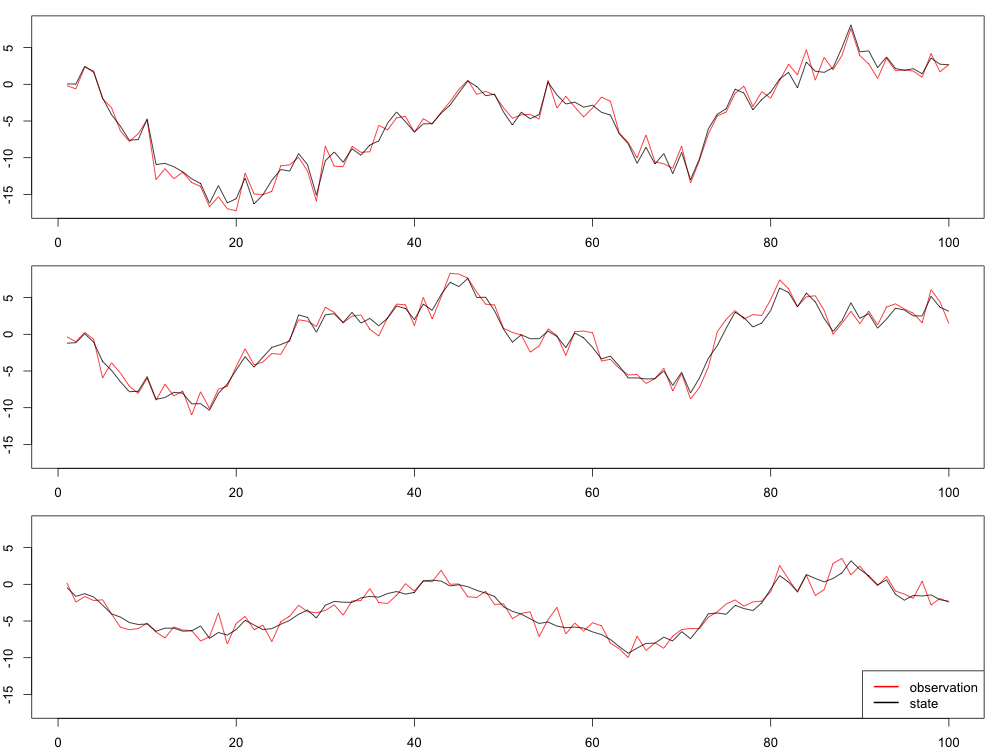
\includegraphics[width=115mm]{../../images/mllm-realization.png}
\caption{Realization of the model with $T=100$}
\label{fig:mllm_realization}
\end{figure}




%%%%  Hierarchical Dynamic Poisson Model   %%%%
\newpage
\section{Hierarchical Dynamic Poisson Model}
Explain the main idea and potential use cases.

\subsection{The Model}
Consider a time series over $M$ days, each consisting of $N$ intra-daily observations. 
Let $m$ denote the day and $n$ be the intraday index.

\bigskip
\begin{center}
\begin{tabular}{ r r l }
  observation: & $y_{mn}$ & $= \text{Poisson}(\lambda_{mn})$\\
  state: & $\log \lambda_{mn}$ & $= \log \lambda_m^{(D)} + \log \lambda_{mn}^{(I)} + \log \lambda_n^{(P)}$\\  
\end{tabular}
\end{center}
\bigskip
where the state consists of a daily, an intra-daily, and a periodic component:
\bigskip
\begin{center}
\begin{tabular}{ r l l }
  daily component: & $\log \lambda_{m+1}^{(D)} = \phi_0^{(D)} + \phi_1^{(D)} \log \lambda_{m}^{(D)}  + \eta_m^{(D)}$ & $\eta_t \sim N(0, \sigma^2_{(D)})$ \\
  intra-daily component: & $\log \lambda_{mn+1}^{(I)} = \phi_1^{(I)} \log \lambda_{mn}^{(I)}  + \eta_{mn}^{(I)}$ & $\eta_{mn} \sim N(0, \sigma^2_{(I)})$ \\
    periodic component: & $\log \lambda_n^{(P)} = \phi_1^{(P)} \sin(\pi (n-1)/M)$ &\\
\end{tabular}
\end{center}
\bigskip
The initial daily and intra-daily component is drawn from a normal with mean $a_1$ and covariance $P_1$: 
$$\log \lambda_{1}^{(D)}, \log \lambda_{1}^{(I)}  \sim N(a_1, P_1)$$ 
Note that both the daily and intra-daily component constitute an AR(1) model, with the mean of the intra-daily component $\phi_0^{(I)}$ set to 0. 
The model is fully specified by the following vector of parameters:
$$
\boldsymbol{\theta} = [ \phi_0^{(D)},  \phi_1^{(D)}, \sigma^2_{(D)}, \phi_1^{(I)}, \sigma^2_{(I)}, \phi_1^{(P)}]^T
$$
Again, the initial state parameters $a_1$ and $P_1$ are assumed to be known.


\subsection{Realization}
\textit{Figure \ref{fig:hdpm_realization}} plots the states and observations for a realization of the hierarchical dyanmic Poisson model over $N=5$ days with $M=20$ intra-daily observations. The model parameters are 
$$
\boldsymbol{\theta} = [ \phi_0^{(D)} = 0.7,  \phi_1^{(D)} = 0.6, \sigma^2_{(D)} = 0.6, \phi_1^{(I)} = 0.3, \sigma^2_{(I)} = 0.2, \phi_1^{(P)} = 0.8]^T
$$
The initial daily and intra-daily state components where drawn from a standard normal.

\begin{figure}[h!]
\centering
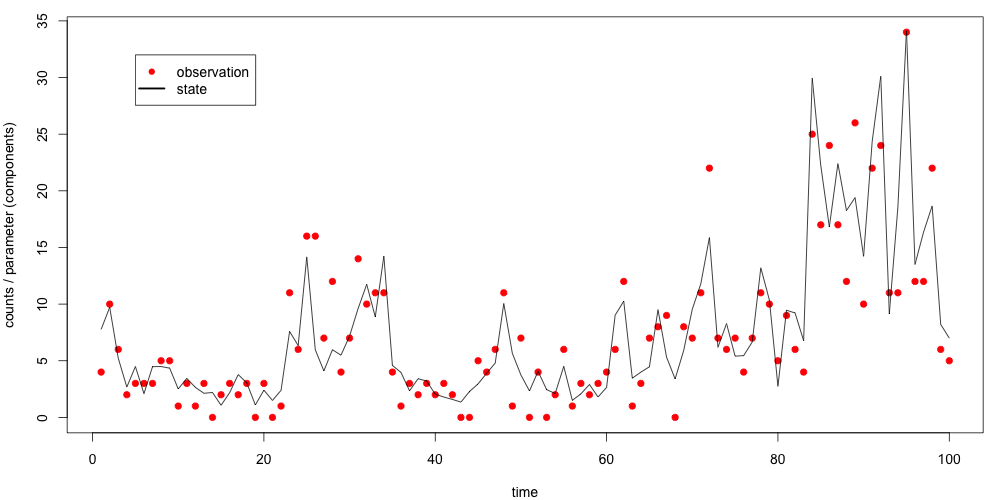
\includegraphics[width=115mm]{../../images/hdpm-realization.png}
\caption{Realization of the model with $N=5$ and $M=20$}
\label{fig:hdpm_realization}
\end{figure}


\subsection{Densities}
State transition and prediction density and how they are used in the particle filter

\subsection{Maximum Likelihood Estimation}
Show log-likelihood plots

\begin{figure}[h!]
\centering
\begin{subfigure}{.5\textwidth}
  \centering
  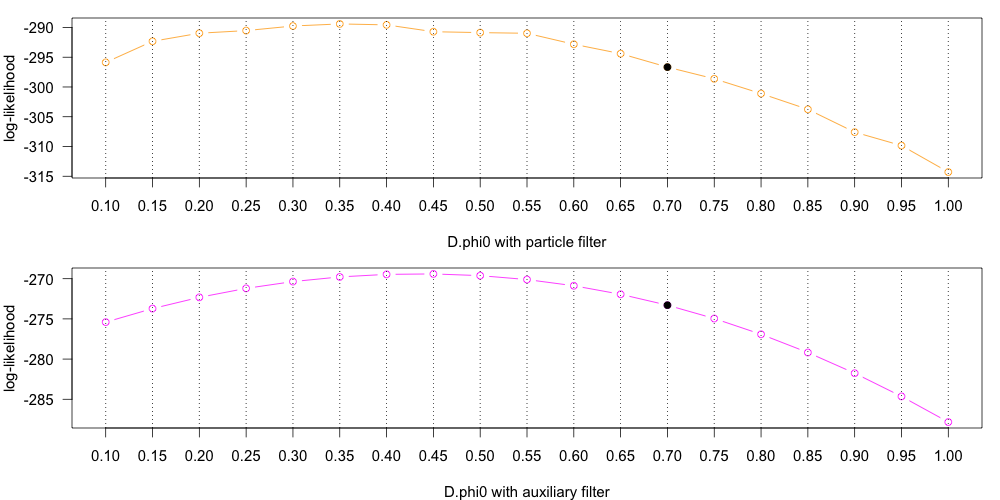
\includegraphics[width=70mm]{../../images/hdpm-loglik-Dphi0.png}
\end{subfigure}%
\begin{subfigure}{.5\textwidth}
  \centering
  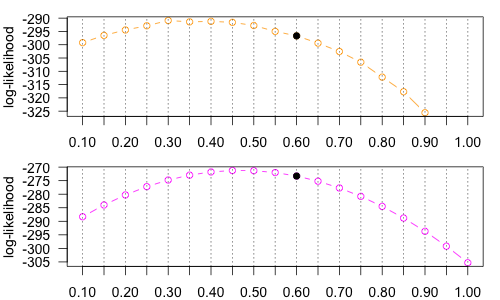
\includegraphics[width=70mm]{../../images/hdpm-loglik-Dphi1.png}
\end{subfigure}
\caption{Belief convergence without misinformation after 300 and 2000 iterations}
\label{fig:conv_nomisinfo}
\end{figure}


%%%%%%%%%%
%    Conclusion   %
%%%%%%%%%%
\chapter{Conclusion}
\label{chp:conclusion}
by Etessami et al.\cite{etessami2014_2}

%%%%%%%%%%%
%    Bibliography          %
%%%%%%%%%%%
%\afterpage{\blankpage}
\bibliography{references}
\bibliographystyle{plain}
\end{document}  















